% Straight up stealing preamble from Eli Holmes 
%%%%%%%%%%%%%%%%%%%%%%%%%%%%%%%%%%%%%%START PREAMBLE THAT IS THE SAME FOR ALL EXAMPLES
\documentclass{article}

%Required: You must have these
\usepackage{Sweave}
\usepackage{graphicx}
\usepackage{tabularx}
\usepackage{hyperref}
\usepackage{natbib}
\usepackage{gensymb}
\usepackage{authblk}

%\usepackage[backend=bibtex]{biblatex}
%Strongly recommended
 %put your figures in one place
 
%you'll want these for pretty captioning
\usepackage[small]{caption}

\setkeys{Gin}{width=0.8\textwidth} %make the figs 50 perc textwidth
\setlength{\captionmargin}{30pt}
\setlength{\abovecaptionskip}{0pt}
\setlength{\belowcaptionskip}{10pt}
% manual for caption http://www.dd.chalmers.se/latex/Docs/PDF/caption.pdf

%Optional: I like to muck with my margins and spacing in ways that LaTeX frowns on
%Here's how to do that
 \topmargin -2cm     
 \oddsidemargin -0.04cm   
 \evensidemargin -0.04cm  % same as oddsidemargin but for left-hand pages
 \textwidth 16.59cm
 \textheight 22.94cm 
 %\pagestyle{empty}       % Uncomment if don't want page numbers
 \parskip 7.2pt           % sets spacing between paragraphs
 %\renewcommand{\baselinestretch}{1.5} 	% Uncomment for 1.5 spacing between lines
\parindent 0pt% sets leading space for paragraphs
\usepackage{setspace}
%\doublespacing

%Optional: I like fancy headers
\usepackage{fancyhdr}
\pagestyle{fancy}
\fancyhead[LO]{How do climate change experiments actually change climate?}
\fancyhead[RO]{2017}
 
%%%%%%%%%%%%%%%%%%%%%%%%%%%%%%%%%%%%%%END PREAMBLE THAT IS THE SAME FOR ALL EXAMPLES

%Start of the document
\begin{document}

% \SweaveOpts{concordance=TRUE}
 \bibliographystyle{/Users/aileneettinger/citations/Bibtex/styles/nature.bst}
\title{How do climate change experiments actually change climate?} 
\author[1,2,*]{A.K. Ettinger}
\author[3]{I. Chuine}
\author[4,5]{B.I. Cook}
\author[6]{J.S. Dukes}
\author[7]{A.M. Ellison}
\author[8]{M.R. Johnston}
\author[9]{A.M. Panetta}
\author[10]{C.R. Rollinson}
\author[11,12]{Y. Vitasse}
\author[1,13]{E.M. Wolkovich}
\affil[*]{Corresponding author: aettinger@fas.harvard.edu}
\affil[1]{Arnold Arboretum of Harvard University, Boston, Massachusetts, 02131, USA}
\affil[2]{Tufts University, Medford, Massachusetts, 02155, USA}
\affil[3]{CEFE UMR 5175, CNRS, Universit\'e de Montpellier,Universit\'e Paul-Val\'ery Montpellier, EPHE, Montpellier, France}
\affil[4]{Lamont-Doherty Earth Observatory, Columbia University, Palisades, New York, 10964, USA}
\affil[5]{NASA Goddard Institute for Space Studies, New York, NY, 10025, USA}
\affil[6]{Department of Forestry and Natural Resources
and Department of Biological Sciences, Purdue University, West Lafayette, Indiana, 47907, USA}
\affil[7]{Harvard Forest, Harvard University, Petersham, Massachusetts, 01366 , USA}
\affil[8]{Department of Organismic and Evolutionary Biology, Cambridge, Massachusetts 02138, USA}
\affil[9]{Department of Ecology and Evolutionary Biology, University of Colorado, Boulder, Colorado, 80309, USA}
\affil[10]{The Morton Arboretum, Lisle, Illinois 60532, USA}
\affil[11]{Institute of Geography, University of Neuch\^atel, Neuch\^atel, Switzerland}
\affil[12]{Swiss Federal Institute for Forest, Snow and Landscape Research WSL, Neuchâtel, Switzerland}
\affil[13]{Department of Organismic \& Evolutionary Biology, Harvard University, Cambridge, Massachusetts, 02138, USA}

%\date{\today}
\maketitle  %put the fancy title on
%\tableofcontents      %add a table of contents
%\clearpage
%%%%%%%%%%%%%%%%%%%%%%%%%%%%%%%%%%%%%%%%%%%%%%%%%%%
%We argue that it is critical for scientists to better understand and report climate from climate change experiments.
%Ben's suggestion: *I just have an overall general comment on the framing of the paper. I think it’s great and would be happy to see it published more or less as is. However, you might consider some rewriting or reorganizing around the two QUESTIONS that I think this paper really gets at:
%	-Did the experimental warming increase the temperature has much as it was supposed to? If not, how off were the treatments from the target warming and why?
%	-What other climate variables (e.g., soil moisture) or statistics (e.g., variability, extremes) change along with the warming treatment?
%Such a reorganization might just make the paper a little more readable and compelling, and give an even firmer narrative hook for the reader to latch onto. Anyway, just my two cents! 
\section* {Preface} %EMW: I think you really need to say what you did here. I basically wanted the sentence that was commented out (but added an alternative version). 
\par Ecological field experiments that alter temperature and precipitation (e.g., with infrared heaters, rain shields, and supplemental watering) are critical tools that scientists use to understand and forecast the biological effects of climate change. These experimental results, however, may be interpreted in misleading ways. The common practice of summarizing and analyzing only the mean changes across treatments hides potentially important variation in treatment effects over space and time. Furthermore, treatments often produce unintended secondary effects, such as soil drying in conjunction with warming, which are rarely fully explored and are likely to have important biological consequences. We assess the magnitude and prevalence of these effects using a new database of daily climate data from 12 experiments. %We demonstrate these points using daily climate data from 12 field-based climate change experiments that use active warming methods. 
%just saw what's wrong- instead of saying what might potentially be wrong
Based on our findings, we present several recommendations for future experimental design, analysis, and data sharing that we believe will improve the ability of climate change experiments to accurately identify and forecast species' responses to changes in climate.
\section* {Introduction}
\par Climate change is dramatically altering earth's biota, shifting the physiology, distribution, and abundance of organisms, with cascading community and ecosystem effects \citep{shukla1982,cox2000,thomas2004,parmesan2006,field2007,sheldon2011,urban2012}. Much uncertainty remains, however, about how particular individuals, populations, species, communities, and ecosystems will respond as shifts in temperature and precipitation regimes become more extreme. Predicting these biological responses to current and future climatic change---and how they will feedback to affect earth's climate and ecosystem services---are among the most significant challenges facing scientists today.

% EMW: I think this paragraph still may need a little work -- we don't spell out for the reader what experiments DO for the first two issues. Lizzie changed a little bit, and this paragraph could be cut down even more. stress what experiments do. 
\par Field-based experiments that alter temperature and precipitation are critical for determining mechanistic links between climate change and biological responses \citep[e.g.,][]{box1978,williams2007,gelman2014}. Such experiments fill in major gaps left by other methods, including observational studies and modeling approaches. Observational studies, which typically correlate recorded biological patterns with measured trends in climate, cannot disentangle the causal effects of warming from other factors that have also changed over time, such as successional stage or land use. Performance of process-based models, which rely on explicit empirical relationships between observed phenomena and climate, can be limited because the underlying assumptions of these models may be poorly constrained \citep [e.g.,][]{pearson2004,ibanez2006,swab2012,chuine2016}. 
In addition, neither approach is well-vetted for predicting future conditions that fall outside the range of historical variability. Climate change has yielded warmer temperatures than the previous 150 years, and possibly warmer than at any time in the last 2000 years \citep{ohlemuller2006,williams2007,williams2007b,ipcc2013}.  

\par Experiments can create these ``no-analog" climate scenarios forecasted for the future, particularly when they employ active warming methods, such as gas-powered forced air heaters, electrical-powered soil warming cables, or infrared heaters \citep{shaver2000,williams2007b,aronson2009}. Active warming is often combined with precipitation manipulations (e.g., snow removal, water additions, or water reductions), and can isolate effects of temperature and precipitation from other environmental changes \citep [e.g.,][]{price1998,cleland2006,sherry2007,rollinson2012}. In addition, if regression designs are used \citep[e.g.,][]{pelini2011} and a range of warming and precipitation treatments are applied, non-linear responses can be estimated. Compared with indoor growth-chamber experiments, field-based experiments offer the possibility of preserving important, but unknown or unquantified feedbacks among biotic and abiotic components of ecosystems. 

\par These experiments are powerful tools, and allow ecologists to draw conclusions about how climate change will affect species' growth, survival, and future distributions \citep{dukes1999,hobbie1999,reich2015,gruner2016}. But is it reasonable to extrapolate findings from these experiments to the real world? Do they actually alter climate in the ways that we think they do? Recent research suggests that climate manipulations do not alter climate in ways that are consistent with observed changes over time \citep{wolkovich2012}. However, a robust assessment of how active warming experiments alter the climate conditions experienced by organisms, and the extent to which these conditions are similar to current field conditions or anticipated climate change, is lacking. 

\par Here, we investigate if and how climate change experiments actually change climate, explicitly looking beyond simple mean shifts. Using plot-level daily microclimate data from 12 active warming experiments (yielding XX experiment years and XX experiment days) we show the direct and indirect ways that climate is altered by experimental manipulations. We highlight the challenges associated with quantifying and interpreting experimental shifts in climate and the resulting biological responses, given that manipulations alter more than mean values. Finally, we use findings from our synthesis to make recommendations for future climate change experiments (Box 1). We focus on \textit{in situ} active warming manipulations, because recent analyses indicate that active warming methods are the most controlled and consistent \citep{kimball2005,kimball2008,aronson2009,wolkovich2012}. The data we use were collected between 1991 and 2014 from North American and European climate change experiments (Figure \ref{fig:map}, Tables S1, S2) and have been merged into a new, publicly available Climate from Climate Change Experiments (C3E) database (see Supplemental Materials for details). 

\section* {Complexities in interpreting experimental climate change} 

Climate change experiments often include detailed monitoring of climate variables at the plot level, yielding large amounts of data, such as daily or hourly temperature and other climate variables, over the course of the experiment. Biologists, however, are generally interested in the biological responses associated with each treatment (e.g., community dynamics, species' growth, abundance, or phenology), which are collected on much coarser timescales (e.g., weekly or annual). Not surprisingly, then, authors typically provide detailed information on the observed biological responses, but report only the mean change in climate over the course of the experiment and whether it matched their target level of change \citep[e.g.][]{price1998,clark2014a,clark2014b,rollinson2012}. 

% This next paragraph is critical -- be sure to include jist of it in cover letter (and consider moving up if we ever change formatting of paper). This contains the main point of the paper. could leave as is
\par Though the published focus is often on shifts in the mean, the imposed climate manipulations actually result in much more complex shifts. The magnitude of change in these manipulations may vary in time and space, and environmental conditions are often unintentionally altered by the presence of the experimental equipment itself. All of these complications challenge our interpretation of how experimental warming studies can be applied to forecast effects of climate change, as discussed below.

\subsection* {Effects on local climate vary over time and space}
Reporting only the mean temperature difference across the duration of the study hides potentially important variations in daily, seasonal, and annual temperatures among treatments. Using the studies included in the C3E database, we found that active warming altered both above-ground and soil diurnal temperature ranges (DTR) in experimental plots, compared with control plots. We observed decreased DTR in above-ground temperatures with active warming compared with controls, perhaps because warming affected maximum temperatures less so than minimum temperatures. We found that active warming increased daily minimum air temperature by, on average, 0.84\degree C per \degree C of warming target, whereas maximum temperature increased only an average of 0.51\degree C per \degree C of target warming (see Supplement Materials). This may be similar to what is projected for parts of the world, since DTR is expected to be altered; however, changes in the DTR will likely vary spatially, as some regions have experienced greater daytime warming than nighttime warming, whereas others have experienced the opposite \citep{ipcc2013}. 

\par In addition to daily fluctuations, there are strong seasonal and annual variations in experimental warming effects (Figure \ref{fig:effwarm}, \ref{fig:blockyear}, Tables S3, S4 in Supplemental Materials). Seasonal variation may occur because treatments are not applied consistently over the year, either because heat applications are frequently shut off during winter months or because some heating methods, even if left on throughout the year, are not capable of applying consistent warming year-round \citep[e.g.][]{clark2014a,clark2014b,hagedorn2010}. For example, seasonal precipitation patterns can alter the effectiveness of warming treatments, since both infrared heaters and soil cables may fail to achieve the target temperatures during rainstorms \citep{peterjohn1993,hoeppner2012}. Wind also has been shown to alter thermal efficiency of infrared heaters, so if heater capacity is limited, target warming levels may not be reached during windy conditions \citep{kimball2005,kimball2008}. Thus, the dramatic inter-annual variation in the amount of effective warming (Figure \ref{fig:blockyear},Table S3) may arise from interactive effects of warming treatments and precipitation, wind, or other aspects of weather that vary annually, as well as seasonally. 

\par Treatment effects also vary spatially, adding further complication to interpreting effects of climate change experiments. The C3E database contains four studies that used blocked designs, allowing us to examine spatial variation in the amount of warming (i.e. the difference between treatment and control plots within a block). We found that the amount of observed warming varied by more than 1 \degree C among blocks (Figure \ref{fig:blockyear}, Table S4); lower warming treatments differed by over 60\% of their target temperature and higher warming treatments differed by over 100\%. 

\par There are numerous potential causes for these differences in warming levels among blocks, given the same warming treatment. Fine-scale variation in vegetation, slope, aspect, soil type, or other factors can alter wind or soil moisture, which in turn affect the thermal efficiency of heaters or other aspects of the warming treatment \citep{peterjohn1993,kimball2005,kimball2008,hoeppner2012,rollinson2015}. %The observed differences in effective warming among blocks highlight the importance of quantifying temperature, soil moisture, and other climate variables at the plot scale, and perhaps within plots, as well. the previous sentence is not necessary- i say too much in the paper already that it is important to think about these things...Condense with the paragraph below. 

% EMW: Let's aim to edit this paragraph (and perhaps the one above) together a little. 
\par %It is, of course, unrealistic to expect experimental treatments to always be consistent at all times and at all spatial scales. 
It's ok that that very: researchers expect variation in the amount of warming at daily, seasonal, and annual scales, as well as across space, as climate change progresses. Already warming rates have varied over space and time \citep{ipcc2013}. However, fine-scale spatial and temporal variations in warming treatments are rarely analyzed explicitly, so the implications for interpretation of experimental findings are unclear. %Isablle: a paper that might be cited here or maybe rather in the discussion regarding repeatabiltiy in ecological expe: Milcu, A., Puga-Freitas, R., Ellison, A. M., Blouin, M., Scheu, S., Girin, T., et al. (in press). Systematic variability enhances the reproducibility of an ecological study. bioRxiv.
% CRR: Is this seasonal precip pattern related to the point about snow cover you mention earlier? I'm wondering if there's some sort of snow or climate threshold where warming has less of an impact. AKE: Could look seasonally at amount of warming to get at this...

\subsection* {Experimental infrastructure alters local climate}
Experimental structures themselves can alter temperature and other important biotic and abiotic variables, in ways that are not generally examined or reported in experimental climate change studies. The importance of having appropriate controls that mimic a treatment procedure without actually applying the treatment is widely acknowledged in biology \citep[e.g.,][]{spector2001,johnson2002,quinn2002}. Though some researchers install treatments with non-functional warming equipment (`sham controls' or `disturbance controls') in experimental climate change studies, the magnitude and implications of structural effects on climate are rarely discussed or interpreted.
\par To investigate the magnitude of infrastructure effects, we compared temperature and soil moisture data from five active warming studies at two sites: Duke Forest and Harvard Forest \citep{farnsworth1995,clark2014a, marchin2015, pelini2011}. These were the only studies in our database that monitored climate in two types of control plots: structural controls (i.e., `shams' or `disturbance controls,' which contained all the warming infrastructure, such as soil cables or infrared heating units but with no heat applied) and ambient controls with no infrastructure added (see Supplemental Materials for details). Other studies monitored environmental conditions in only structural controls (n=3) or only ambient controls (n=4).

\par We found that experimental structures altered above-ground and soil temperatures in opposing ways: above-ground temperatures were higher in the structural controls, compared with ambient conditions with no structures installed, whereas soil temperatures were lower in the structural controls compared with ambient soil (Figure \ref{fig:shamamb}a,b, Tables S5-S10). This general pattern was consistent across the different temperature models we fit (mean, minimum, and maximum temperatures), although the magnitude varied across seasons (Figure \ref{fig:shamamb}a,b), as well as among studies, years, and with ambient temperature (Tables S5-S10). In addition, soil moisture was lower in structural controls compared with ambient conditions (Figure \ref{fig:shamamb}c, Tables S7, S10). 

\par There are several possible reasons for the observed differences between ambient and structural controls. Infrastructure materials may shade the plots, reduce airflow, reduce albedo relative to surroundings, or otherwise change the energy balance. Structures could also interfere with snow accumulation, thereby reducing snowpack and its insulation. This likely plays a bigger role in soil temperature differences at the Harvard Forest sites (exp04, exp07, exp08), where average snowfall is over one meter, than at Duke Forest (exp03,exp10), where average snow accumulation each winter is 20 cm or less. Although we could find very little discussion of measured temperature (or other) differences between ambient and structural control plots in most previously published work \citep[e.g.,][]{farnsworth1995,pelini2011,clark2014a,clark2014b}, Clark \textit{et al.} (2014) do mention that ``control of the air temperature was less precise, in part due to air scooping on windy days." Marchin \textit{et al.} (2015) also note that structural controls had mean spring air temperatures about  0.5\degree C or more above ambient temperatures. Peterjohn \textit{et al.} (1994) reported cooler soil temperatures in structural versus ambient control plots, but only at shallow soil depths (4 cm deep, in their study). Similarly, in our analysis we found the greatest difference between soil temperature in sham and ambient controls to be in exp10, one of the two studies in which temperature was measured at depths of 2 cm (the other was exp07), rather than 15 cm deep (exp03 and exp04). 

\par In addition to the structural effects that we document here on temperature and moisture, experimental structures may alter conditions by altering herbivory and other biotic interactions \citep{kennedy1995,moise2010,wolkovich2012,hoeppner2012}. Most warming experiments to date deal with this by calculating focal response variables relative to ambient controls to account for the infrastructure effects \citep [e.g.,][]{marchin2015}. Further documentation and analysis of the effects on abiotic and biotic factors, as well as in depth interpretation of how these effects may alter focal variables, is an important next step for climate change experiments, particularly if we wish to use results for forecasting.

\section* {Secondary and tertiary effects of climate change manipulations} 
Climate change experiments often seek to manipulate one or two climate variables, such as temperature and precipitation. However, non-target abiotic and biotic factors may also be affected by these manipulations. For example, precipitation treatments typically reduce temperatures in climate change manipulations \citep{sherry2007,rollinson2012,mcdaniel2014}: McDaniel et al. (2014) observed that a twenty percent increase in precipitation reduced mean hourly temperatures by 0.3\degree C over the course of their two-year experiment.

\par Experimental warming typically increases vapor pressure deficit and reduces soil water content (Figure \ref{fig:mois}) \citep[e.g.,][]{sherry2007,morin2010,templer2016}. Of the twelve experiments in the C3E database, we examined the ten that measured and reported soil moisture and found that soil moisture was reduced by 3.0\%, on average, in warmed compared with ambient plots (Table S12); this reduction occurs at a rate of 0.43\% per degree of target warming (Table S11). Thus, although active warming experiments often do not manipulate soil moisture directly, soil moisture is unavoidably affected by changing temperatures. % To examine the effects of warming treatment on soil moisture, we fit linear mixed effects models to data from these ten sites (see Supplement for details). 

% EMW: I think the below would be better if you said: multiple studies have found a shift towards woody vegetation (Rollinson, Harte) .... I think the paper still has a few too many 'for examples' especially given that you have a thorough synthesis to report. 
\par Warming and precipitation treatments, and their indirect effects on soil moisture and other abiotic factors can also alter the biotic environment, which may feed back to produce tertiary effects that also alter climate. Many studies have found shifts in plant and micropbial composition (Rollinson, Harte). These shifts in composition may change competitive dynamics and, in turn, affect resource levels, such as moisture and carbon in the soil \citep{harte2015}. In addition, warming reduces soil water content and alters soil microbial communities, which can also affect available nutrients \citep{mcdaniel2014,mcdaniel2014b}. %The magnitude of all of these effects are likely to vary in space and time; some may be transient whereas others may be more permanent.

% EMW: Is this supposed to be a paragraph on its own? Also, possible to delete or shorten first sentence?
%Clearly, it can be difficult to tease apart the specific abiotic and biotic drivers of temperature and other climatic changes that occur in experimental treatments. , however. 

\par The widespread presence of unintended secondary effects of climate change manipulations highlights the importance of measuring environmental conditions at the plot level, and using these measurements in data analysis and interpretation of results. Many climate change experiments (seven of the 12 in the C3E database, for example) model warming and/or precipitation treatments as categorical predictors (and in some cases, orthogonal crossed treatments, when both treatments are included in the experiment, i.e., a traditional repeated measures, three-way ANOVA). Understanding these interrelated drivers is critical for determining mechanistic explanations for observed responses to warming.

\par The interacting and secondary effects of these manipulations, as well as the plot-level variation in warming effectiveness and effects of experimental structures on temperature and soil moisture that we discuss above, demonstrate a clear need for an alternative modelling approach to fully understand the experimental results. One option is to include the continuous climate data (e.g., plot-level mean temperatures), as a predictor of the focal response variable, such as phenological state or species density \citep [e.g.,][]{marchin2015, pelini2014}. A challenge with this approach is that much of the true variation in the climate is lost through aggregation (e.g., calculating mean annual or seasonal temperature), and the chosen method of aggregation affects both the mean and variance of the climate estimate \citep [e.g.,][]{clark2014b}. 

\section* {Biological implications}

\par We have highlighted a suite of factors that complicate interpretation of warming experiments. These largely unintended alterations are likely to have biological implications, including for many of the major responses studied in warming experiments, such as plant phenology (Figure \ref{fig:biolimp}). Interpretation of experimental climate change effects on biological responses may be misleading, because the intended climate treatments (i.e. categorical comparisons or target warming levels) are generally used as explanatory variables in analyses. The interpretation is likely to be altered by using fine-scale, measured climate as the explanatory variables (e.g., plot-level temperature and soil moisture), because detailed examination of multiple microclimate variables will allow a more complete understanding of the indirect, as well as direct, effects of applied treatments on abiotic and biotic drivers of focal responses.

\par Plant phenology provides one example of a biological response that is muted in experiments versus observational studies (Figure \ref{fig:biolimp}b). This is because phenology is likely to be altered in opposing ways by the direct effects of increased air temperatures---which generally advance phenology \citep{wolkovich2012}---and the indirect effect of decreased soil moisture---which may delay phenology or at least reduce advancement due to warming \citep{penuelas2004,ourcival2011,craine2012,matthews2016}. 
These opposing drivers may be responsible for the observed discrepancy between observational and experimental phenological responses to warming \citep{wolkovich2012}. Other biological responses may be exaggerated in experiments when direct and indirect effects of climate manipulations work in concert (Figure \ref{fig:biolimp}c). Accounting for indirect, as well as direct, effects of warming is critical for accurate interpretation about the consequences of climate change \citep{kharouba2015}. Since climate change experiments have indirect effects on the biotic as well as abiotic environment \citep{hoeppner2012,pelini2014,diamond2016}, a critical question is the extent to which these indirect effects are accurate forecasts of future shifts that are likely to occur with climate change, or due to side-effects that are unlikely to occur outside of experimental systems \citep{moise2010,diamond2013}.
\section* {Conclusions}
 \par Climate change experiments provide invaluable information about biological responses to climate change, yet the full range of changes in environmental conditions imposed by these experiments is rarely presented. We believe the data we have compiled in the C3E database, as well as the complications we have highlighted, provide a foundation for designing better experiments and gaining the most knowledge and utility from existing experiments. We also recognize that funding levels, time, and logistical issues often constrain researchers' abilities to monitor and analyze a larger suite of environmental conditions in climate manipulations. However, we argue that these data have value for the broader research community, and that they should be collected and made public when possible. In Box 1, we describe specific recommendations to improve implementation, interpretation, and communication of the results of climate change experiments in the future. % EMW: If you need space, you could cut this last sentence and just add (see Box 1) to the end of the last sentence. % Me again! I think the last three sentences should be condensed to one short one. This is a really long conclusion section. 
Condense the previous paragraph with this one:
Say: Funding levels will always be an issue, but this is critical
 
 \par Researchers have been studying the implications of climate change for ecosystems for nearly four decades \citep[e.g.,][]{tamaki1981,carlson1982}.
Yet, as climate change across the globe continues with projected warming likely to exceed 2 \degree C over the next 80 years \citep{ipcc2013}, ecologists are challenged to not only document impacts but make quantitative, robust predictions. Our ability to meet this challenge requires building on the data from current and past experiments to better understand how changes in climate alter ecological processes, and to design better experiments in the future. To facilitate this, we have compiled the first database of fine-scale climate data from multiple warming experiments and shown how time, space, and experimental artifacts may hinder simple interpretations of climate change experiments. 

\par The next steps require the ecological community to evaluate their data in new ways. We can then build on these data to develop and use novel approaches in future experiments. This will allow researchers to more accurately and confidently elucidate mechanisms underlying biological responses and feedbacks.
\section* {Box 1: Recommendations for future climate change experiments} 
\begin{enumerate}
\item\textit{Collect and analyze fine-scale climate data.} This includes analyzing and interpreting minimum and maximum values, as well as variance and critical thresholds (e.g., the number and duration of freeze-thaw events and accumulated chilling hours) \citep{mcdaniel2014,vasseur2014}. We suggest saving the raw data from data loggers (often collected at hourly or higher resolution) to allow quantification of variance (and other summaries) at different temporal resolutions. In assessing which frequency of measurements is most appropriate for analyses (e.g., hourly, twice daily), it is critical to consider the chronobiology of the event and organisms of interest. For ants, this might mean that temperatures be monitored every minute \citep{shavit2017}; for bacteria, even more frequently. Although this recommendation requires large and potentially cumbersome data files, recent advances in data standards and remote-storage repositories make this a more feasible request now than when these warming experiments began. % EMW: Cut last sentence if space needed?
\item\textit{Analyze measured climate variables rather than targets}. There can be substantial variation in the effects of warming and precipitation treatments among plots and across time (Figure \ref{fig:blockyear}). Furthermore, these applied climate treatments are not independent: precipitation treatments alter the effectiveness of warming, and warming treatments alter available moisture levels. Analyzing measured climate will allow much more in-depth understanding of the drivers and the biological effects of variation in temperature and moisture. % EMW: Cut second sentence if needed.
% EMW: Below is way too long, cut in half?
\item\textit{Publish high quality, usable data and metadata} such that data can easily be easily re-used. Include detailed data about experimental treatments, such as the number and cause of missing data points for climate, the timing of applied warming treatments (i.e., exact start and end dates, within and across years). Given that experimental in situ active climate manipulations are logistically challenging and expensive \citep{aronson2009}, and that they often produce a large volume of fine-scale climate data, good curation and data sharing will ensure wider use and more in-depth understanding of these valuable data. When studying biological implications of a global challenge as large as climate change, progress will come from designing, running and reporting experiments in ways that facilitate an eventual global data set. We found that studies reported a diverse range of climate variables, collected in different ways (Table S2). It is a challenge to synthesize these diverse data, and to tease apart whether variable findings are due to methodological differences, to measurement error, or to true variation in biological responses. %EMW: Cut or move the last two sentences?
\item\textit{Include both structural and ambient controls} and collect, use, and report data collected within them. Fewer than half of the studies in our C3E database included these two control types (5 out of 12); however, all experiments showed significant effects of infrastructure. Future consistent monitoring of all climate and biological variables in both control types will enable scientists to tease apart mechanisms due to experimental design from mechanisms due to shifts in climate. To date, these side effects are rarely reported or interpreted in climate change experiments, but our analyses suggest they are ``demonic intrusions" that should be considered, and reduced when possible \citep{hurlbert1984}. %EMW: Reduce last two sentences a lot. 
\item\textit{Design relevant manipulations} by consulting observational records and forecasts, including seasonal variation in projected warming. If the goal is to mimic future climate conditions, careful consultation of climate change projections, as well as historical data, for the study region can aid in selection of warming and precipitation treatment methods that most closely mimic anticipated changes. When it is not possible or desirable to match anticipated changes in climate, studies should report how imposed treatments compare to projected changes and/or past observations \citep[see, e.g.,][]{hoover2014}. In addition, the timing of the imposed treatments should be carefully considered. When continuous treatments are not applied throughout the study, the seasonality and timing of treatments should be explicitly reported and the climate should be monitored throughout, even when no manipulations are implemented.
% EMW: Below, I would contrast Gruner ref with other (non-warming) studies where results do change over time, biodiversity studies for example... 
\item\textit{Maximize the duration of climate change experiments} by running some experiments for as long as possible. Though there is little evidence that study duration affects biodiversity responses in warming experiments \citep{gruner2016}, long-term responses of individuals and populations can differ from transient responses \citep{saleska2002,franklin1989,giasson2013,harte2015}. Teasing apart exactly when long-term studies are required needs further investigation. Understanding a long-term process like climate change will require investment in some long-term experiments, while also balancing the need for shorter-term studies in more locations. Well-designed and well-supported longer warming experiments will allow study of how inter-annual variations interact with climate change treatments, especially when looking at non-linear and multi-year processes. 

\end{enumerate}
\bibliography{/Users/aileneettinger/citations/Bibtex/mylibrary}
\clearpage

\section* {Figures}


\begin{figure}[p]
\centering
\includegraphics{../Analyses/maps/RadcliffeLocations_Experiments.png} 
\caption{\textbf{Climate data from 12 climate change experiments in North America and Europe are included in the C3E database and analyzed here.} See Tables S1, S2 in the Supplemental Materials for details.} 
 \label{fig:map}
 \end{figure}
\clearpage
\begin{figure}[h]
\centering
 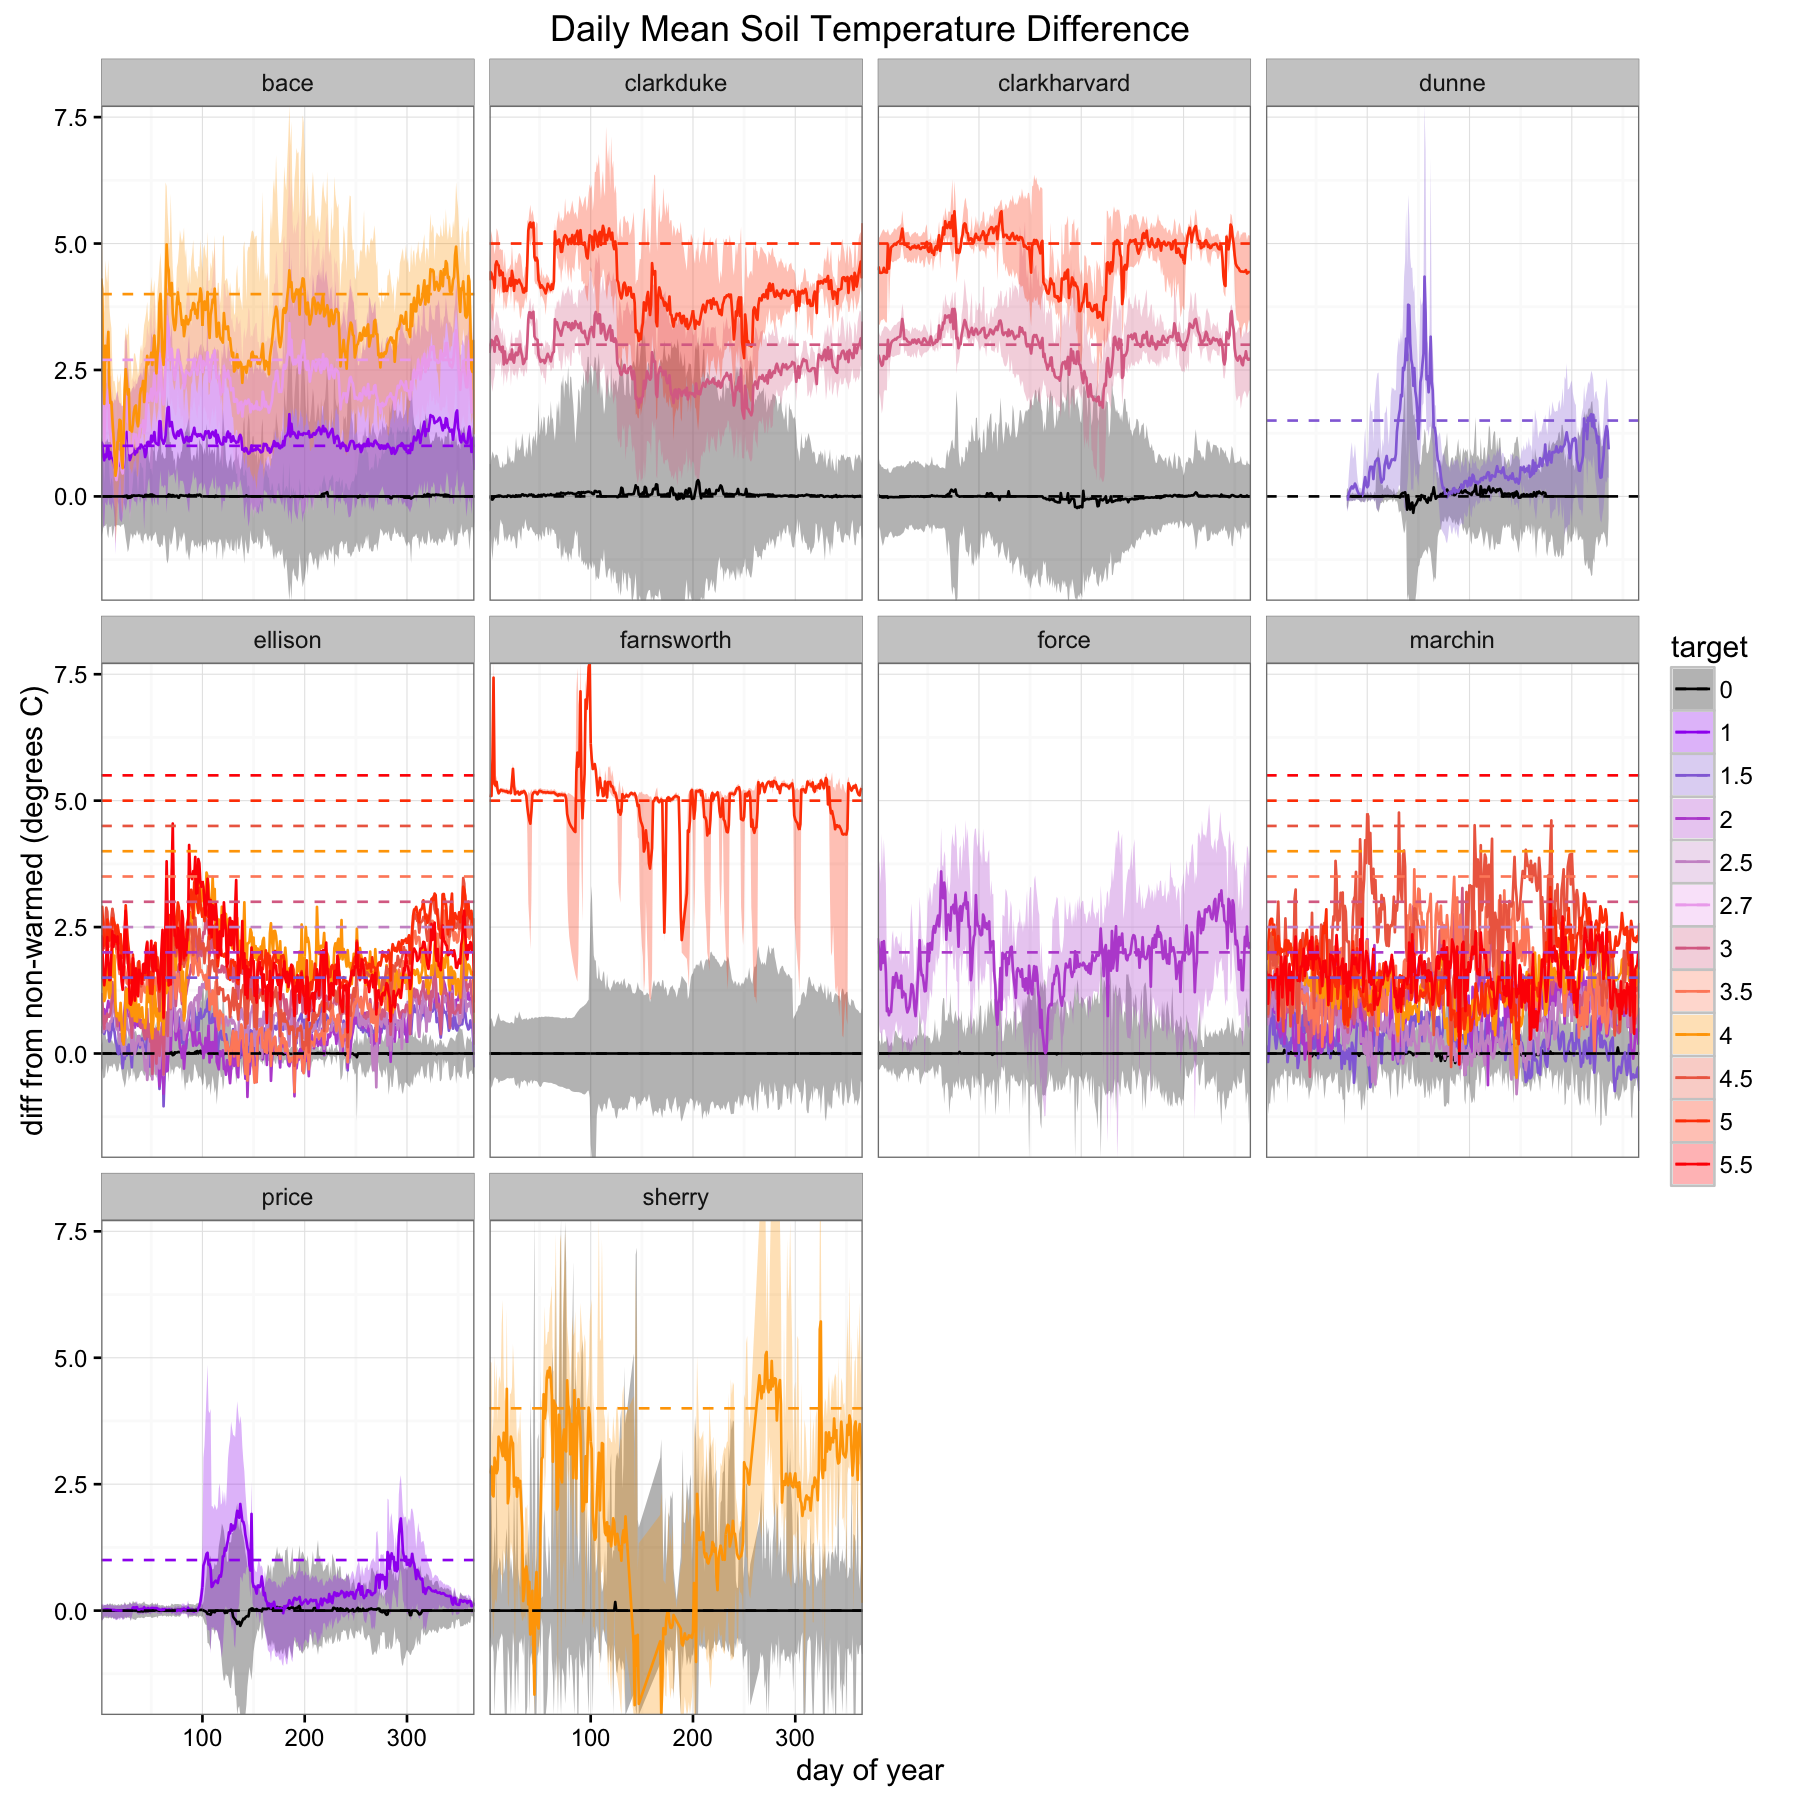
\includegraphics{../Analyses/figures/Exploratory_TimeSeries_SoilTemp1Mean_Deviation.png}
 \caption{\textbf{Deviations in daily observed warming from mean soil temperature are shown for 10 study sites.} Black lines represent control plots, and colored, dashed lines represent warming treatments with various target warming levels (ttwo sites not shown here did not monitor soil temperature). Sites exp07 and exp10 used a regression design, with target warming for each chamber ranging from 1.5 to 5.5 \degree C. Daily temperature values were obtained by averaging across years for each day of the year in each plot in each study. We then averaged across plots to get the mean line and 95\% confidence intervals (shaded areas), which therefore represent the variability in treatment effectiveness based on the replicates. Mean annual temperature for the experimental site is shown in the upper right corner of each plot, and plots are arranged by increasing mean annual temperature.}
 \label{fig:effwarm}

 \end{figure}
 \begin{figure}[p]
   \centering
 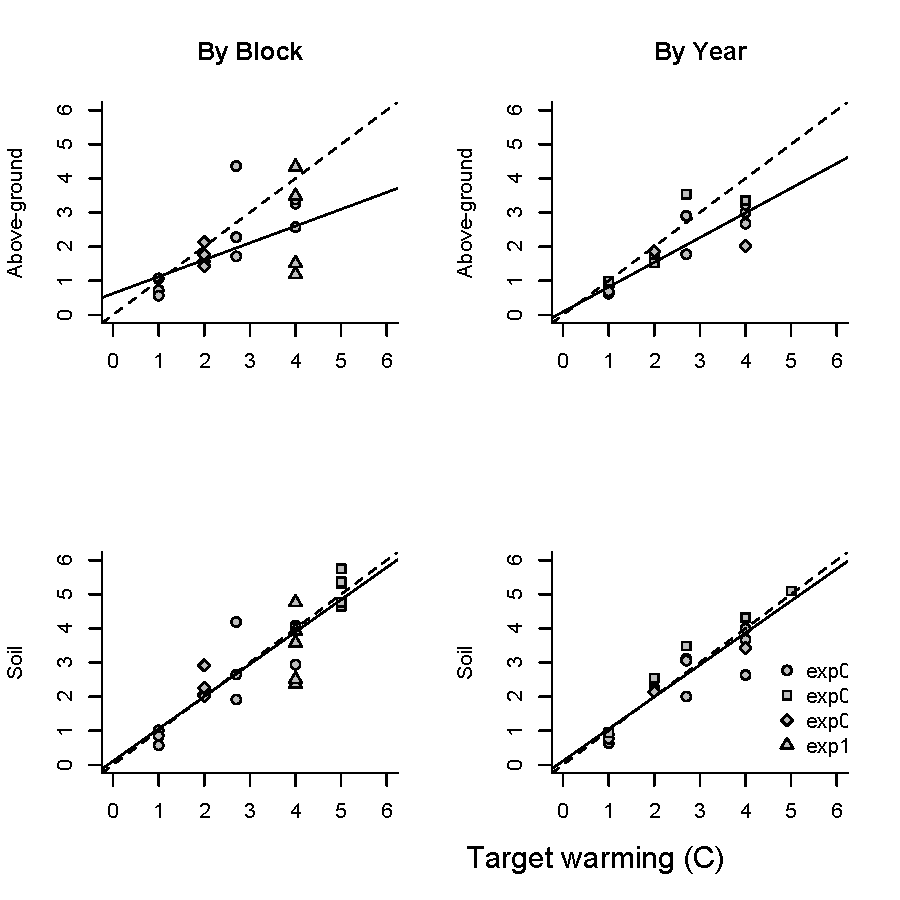
\includegraphics{../Analyses/figures/blockyearvar.pdf}  
 \caption{\textbf{Observed warming (i.e. the difference between treatment and control plots) over space and time, for above-ground and below-ground temperatures.} The solid line is the fitted relationship between target and observed warming, using a linear mixed effect model with a site random effect, and the dashed line shows when observed warming is exactly equal to target warming (1:1). Left panels show spatial regressions, in which the amount of observed warming by block is the difference between treatment and control plots within each block, across all years that a study was conducted. Right panels show temporal regression, in which the amount of warming by year is the difference between treatment and control plots within a year, across all blocks in a study. Four of the 12 studies in the C3E database used blocked designs, and data from these studies are shown here. See Supplemental Materials for statistical details.}
 \label{fig:blockyear}
 \end{figure}
 \clearpage
 
 
 \begin{figure}[p]
\centering
 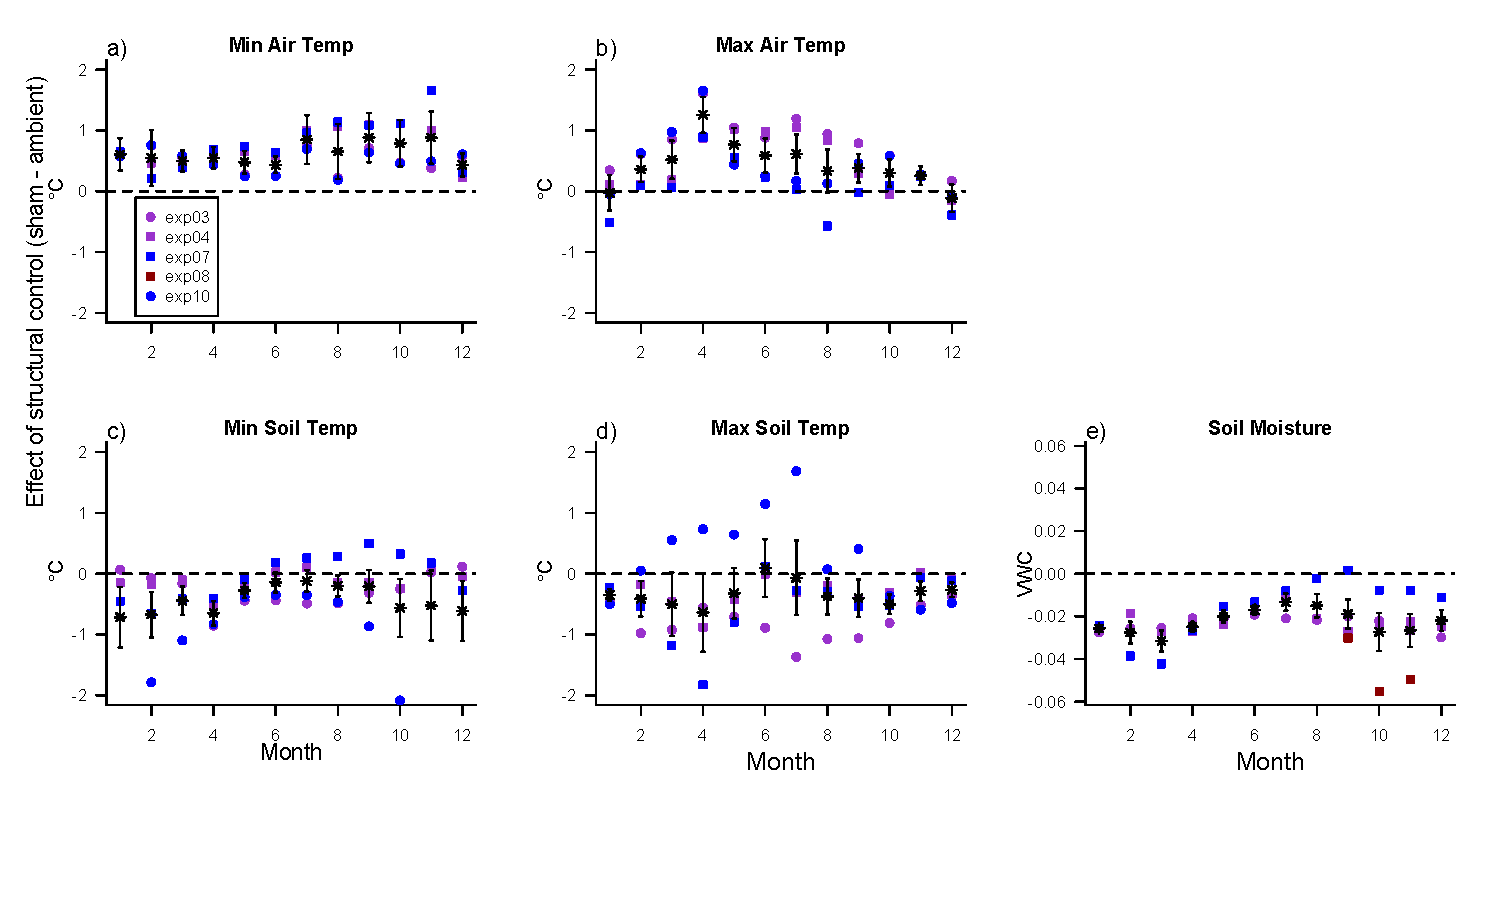
\includegraphics{../Analyses/figures/ShamVSAmbient_all.pdf}  
 \caption{\textbf{Deviations in measured abiotic variables by month in structural versus ambient controls} (i.e. with no control chambers or warming infrastructure in place). Above-ground temperatures were higher, whereas below-ground temperature and soil moisture were lower in structural controls compared with ambient controls. We show fixed effects (in black) from monthly mixed effects models that account for differences in experimental design and other factors among sites by including site and year (nested within site) as random effects (see Tables S5-S10 in Supplemental Materials for details). Site-level random effects are shown by symbols in blue (for the three studies conducted at Harvard Forest in Massachusetts, USA) and pink (the two studies conducted at Duke Forest in North Carolina, USA).}
 \label{fig:shamamb}
 \end{figure}
\clearpage
 \begin{figure}[h]
    \centering
 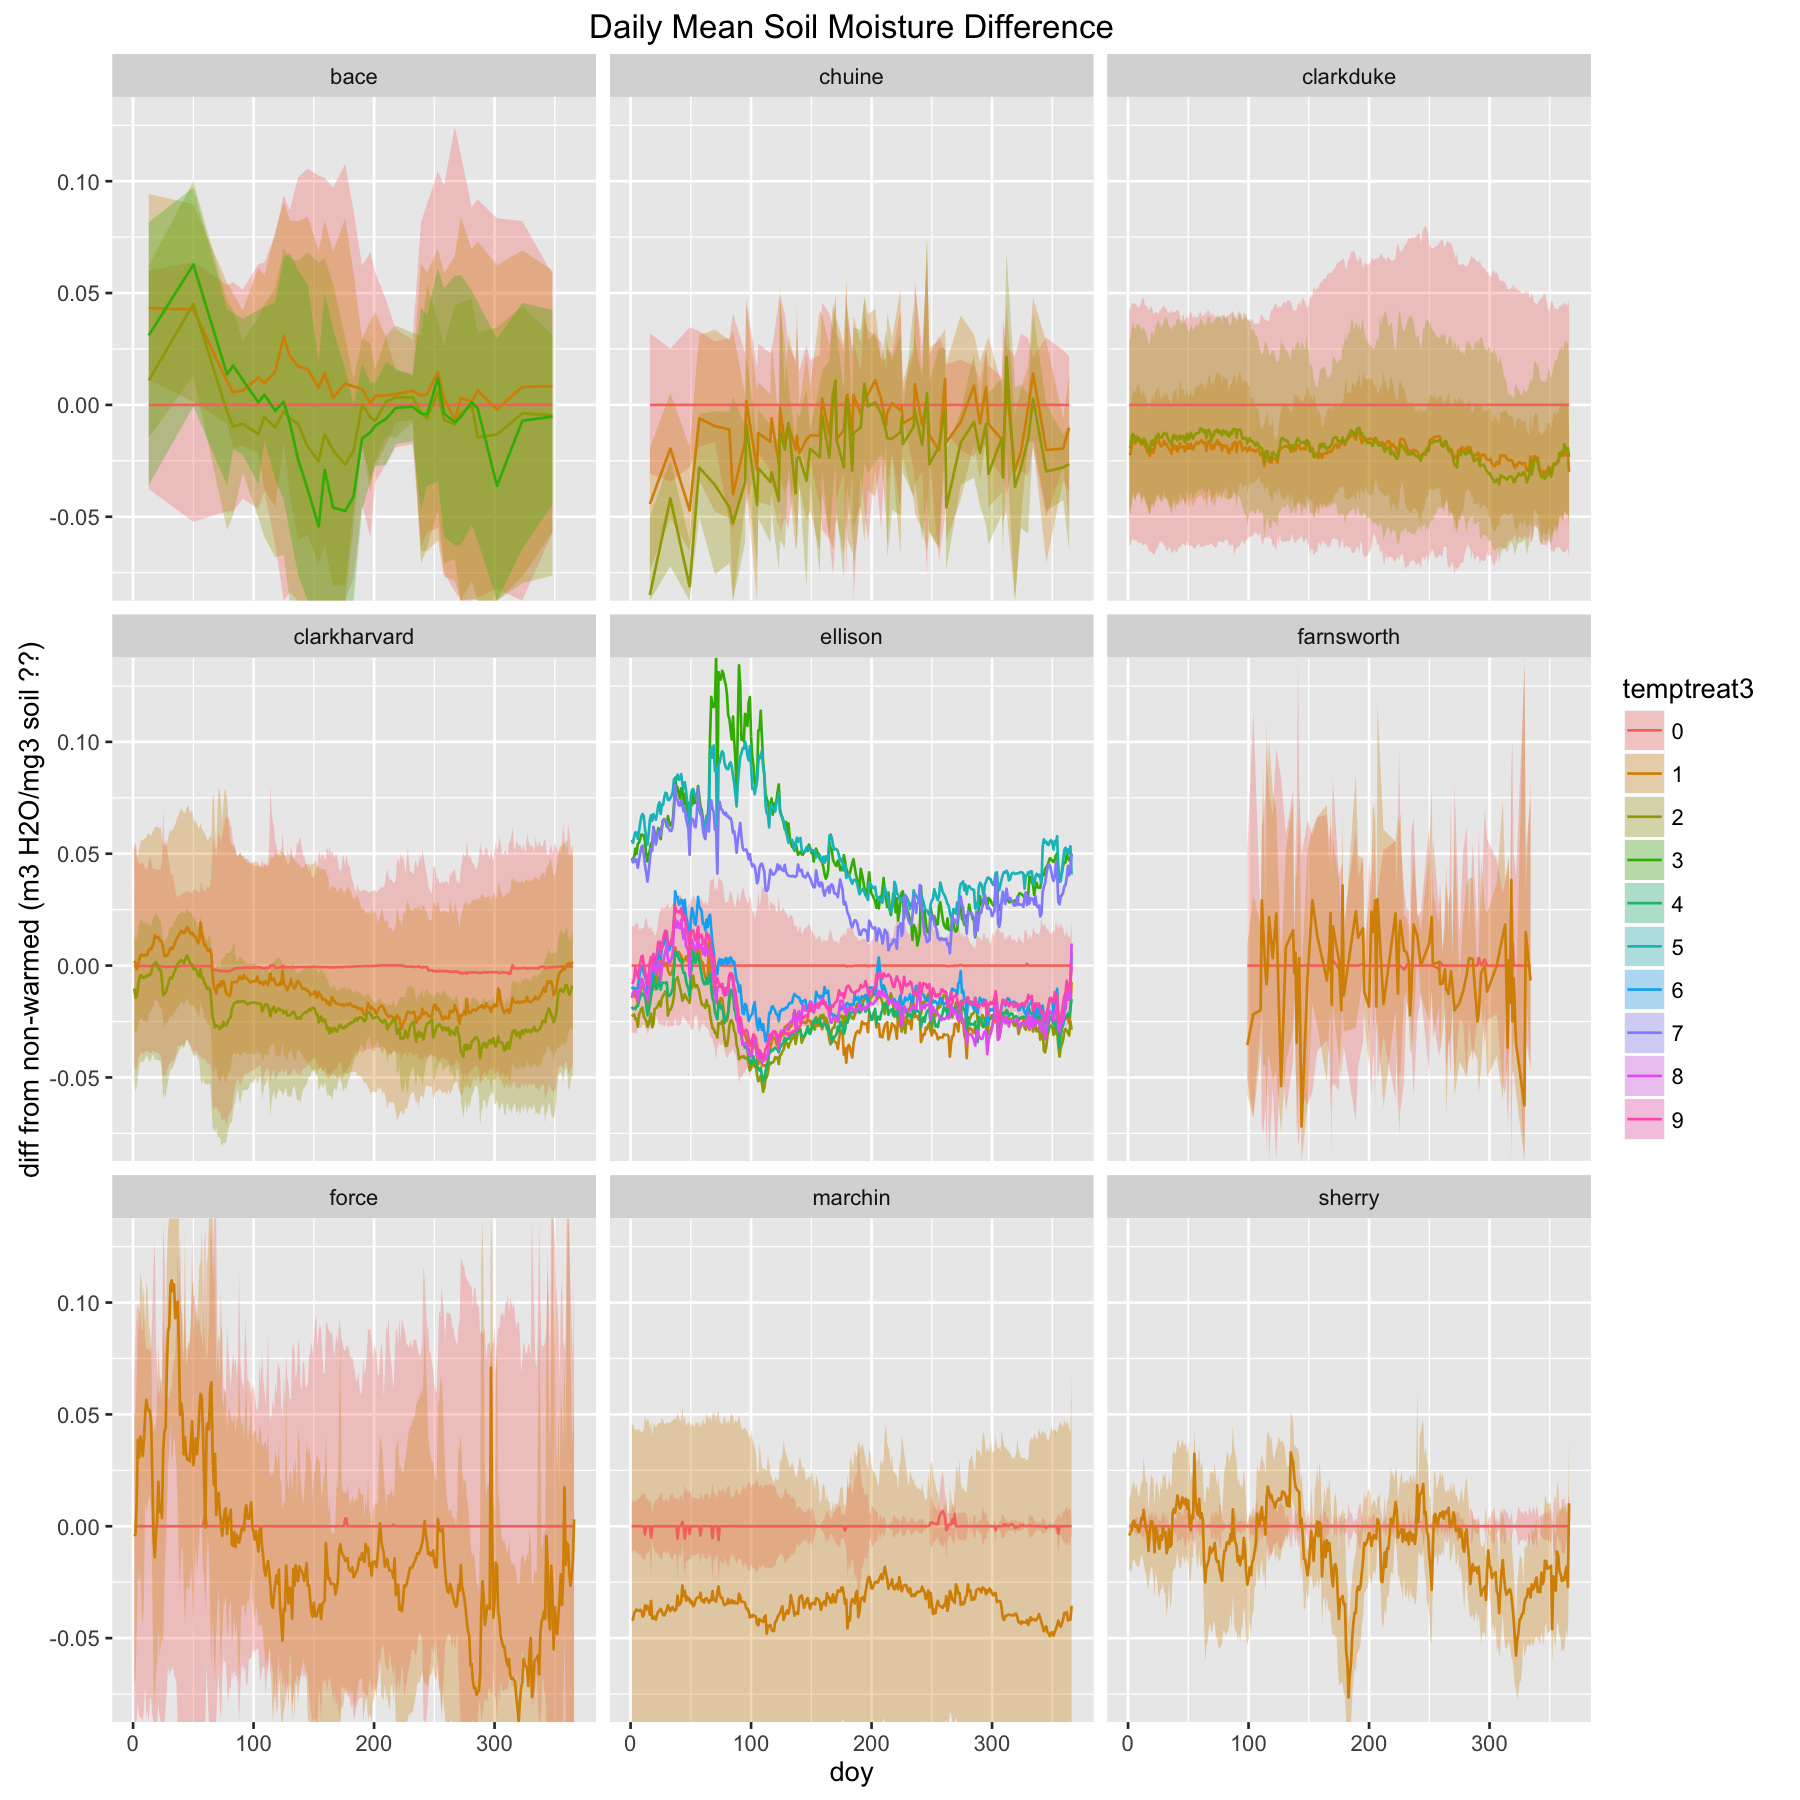
\includegraphics{../Analyses/figures/Exploratory_TimeSeries_SoilMoist_Deviation.png}  
 \caption{\textbf{Deviations in daily observed soil moisture,} shown for the nine  study sites that continuously monitored soil moisture. Black lines represent control plots, and colored, dashed lines represent warming treatments with various target warming levels. Sites exp07 and exp10 used a regression design, with target warming for each chamber ranging from 1.5 to 5.5 \degree C. Mean annual moisture for the experimental site is shown in the upper right corner of each plot, and plots are arranged by increasing mean soil moisture}. %ISabelle: yaxis for our experiment was m3 H2O per m3 soil
 \label{fig:mois}
 \end{figure}
 \begin{figure}[h]
 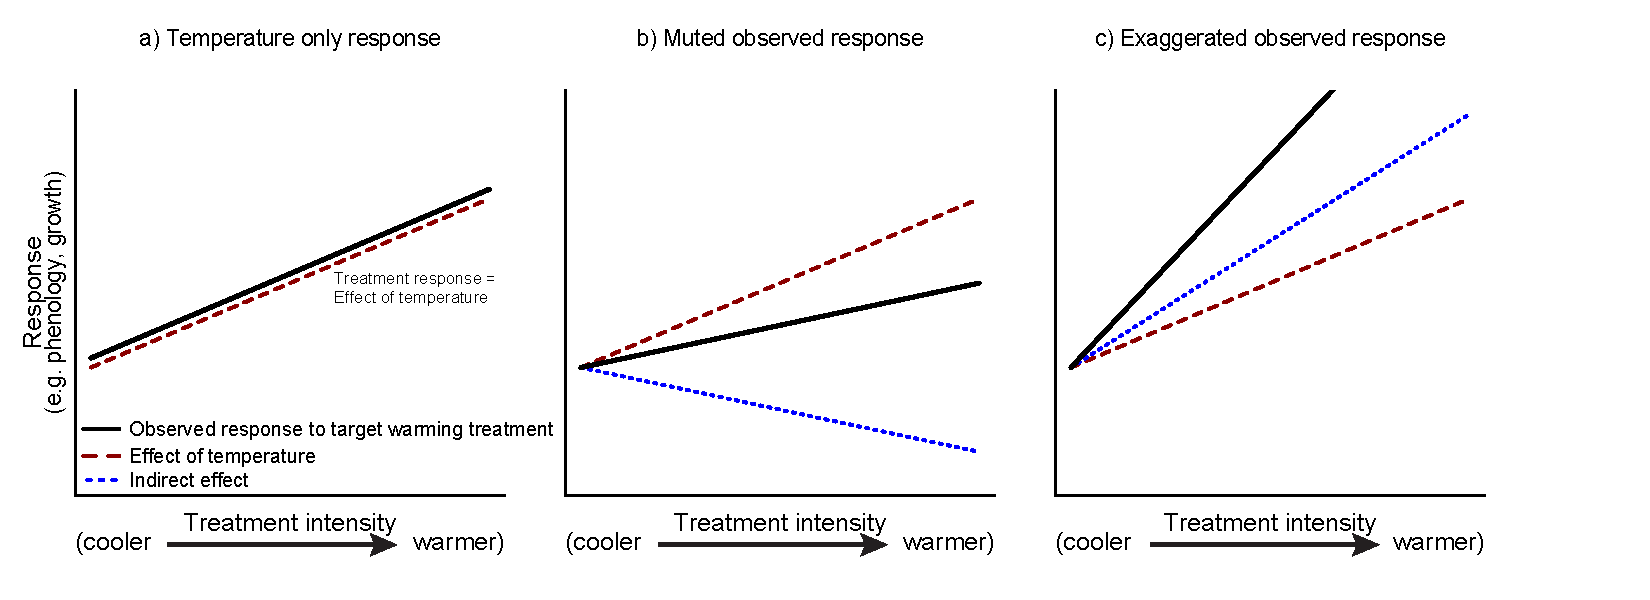
\includegraphics{../Analyses/figures/DirIndWarmingEffects.pdf} 
 \caption{\textbf{Possible biological responses to experimental climate change and their interpretation}. Direct responses to temperature alone (a) can be easily understood. Complications arise when biological responses are a mix of the direct and indirect effects of experimental warming. Then experimental warming may cause biological responses to be muted (b) or exaggerated (c). Slopes of these example lines assume that direct and indirect effects are additive; however, the relationship between these effects could be more complex (e.g., antagonistic, multiplicative, or otherwise interactive).} 
\label{fig:biolimp}
  \end{figure}
%%%%%%%%%%%%%%%%%%%%%%%%%%%%%%%%%%%%%%%%
\end{document}
%%%%%%%%%%%%%%%%%%%%%%%%%%%%%%%%%%%%%%%%
